\documentclass[xcolor={table}]{beamer}
\usepackage{fleqn}
\usepackage{graphicx}
\usepackage{coordsys} %for \numbline commander

%Setup appearance:
\usetheme{Darmstadt}
%\usefonttheme[onlylarge]{structurebold}
\usefonttheme{professionalfonts}
\setbeamerfont*{frametitle}{size=\normalsize,series=\bfseries}
\setbeamertemplate{navigation symbols}{}
\setbeamertemplate{bibliography item}{[\theenumiv]}

% Standard packages
\usepackage[english]{babel}
\usepackage[latin1]{inputenc}
\usepackage{times}
\usepackage[T1]{fontenc}
\usepackage{multirow}
\usepackage{subfigure}
\usepackage{pbox}
\usepackage{arydshln}
\usepackage{pifont}
\usepackage{cancel}
\usepackage{rotating} % for sideways headings

% Source Code packages
\usepackage{algorithm2e}
\usepackage{algorithmic}

\DeclareSymbolFont{extraup}{U}{zavm}{m}{n}
\DeclareMathSymbol{\varclub}{\mathalpha}{extraup}{84}
\DeclareMathSymbol{\varspade}{\mathalpha}{extraup}{85}
\DeclareMathSymbol{\varheart}{\mathalpha}{extraup}{86}
\DeclareMathSymbol{\vardiamond}{\mathalpha}{extraup}{87}

%%% This section command that adds a big page with section dividers
\usepackage{xifthen}% provides \isempty test
\newcommand{\SectionSlide}[2][]{
	\ifthenelse{\isempty{#1}}
		{\section{#2}\begin{frame} \begin{center}\begin{huge}#2\end{huge}\end{center}\end{frame}}
		{\section[#1]{#2}\begin{frame} \begin{center}\begin{huge}#2\end{huge}\end{center}\end{frame}}
}
%Extends the section slide to to include a shortened section title for the navigation bar as a second parameter
\newcommand{\SectionSlideShortHeader}[3][]{
	\ifthenelse{\isempty{#1}}
		{\section[#3]{#2}\begin{frame} \begin{center}\begin{huge}#2\end{huge}\end{center}\end{frame}}
		{\section[#1]{#2}\begin{frame} \begin{center}\begin{huge}#3\end{huge}\end{center}\end{frame}}
}

\newcommand{\refer}[1]{\footnote{#1}}
\newcommand{\GW}{\text{\textit{Guess-Who~}}}
\newcommand{\keyword}[1]{\alert{\textbf{#1}}\index{#1}}
\newcommand{\firstkeyword}[1]{\textbf{#1}\index{#1}}
\newcommand{\indexkeyword}[1]{\textbf{#1}\index{#1}}
\newcommand{\featN}[1]{\textsc{#1}}
\newcommand{\featL}[1]{\textit{'#1'}}
 \newcommand{\ourRef}[1]{\ref{#1} $^{\text{\tiny[\pageref{#1}]}}$}
 \newcommand{\ourEqRef}[1]{\eqref{#1}$^{\text{\tiny[\pageref{#1}]}}$}
  
\DeclareMathOperator*{\argmax}{argmax}
\DeclareMathOperator*{\argmin}{argmin}

\title{Machine Learning for Predictive Data Analytics}
	\author{John D. Kelleher and Brian Mac Namee and Aoife D'Arcy}
	\institute{}
	\date{}
\begin{document}
\begin{frame}
	\titlepage
\end{frame}
\begin{frame}
	 \tableofcontents
\end{frame}

\SectionSlideShortHeader{What is Predictive Data Analytics?}{Predictive Data Analytics}

 \begin{frame} 
\begin{itemize}
	\item Predictive Data Analytics encompasses the business and data processes and computational models that enable a business to make \keyword{data-driven decisions}.
\end{itemize}
\end{frame} 


 \begin{frame} 
\begin{figure}[htb]
       \begin{centering}
       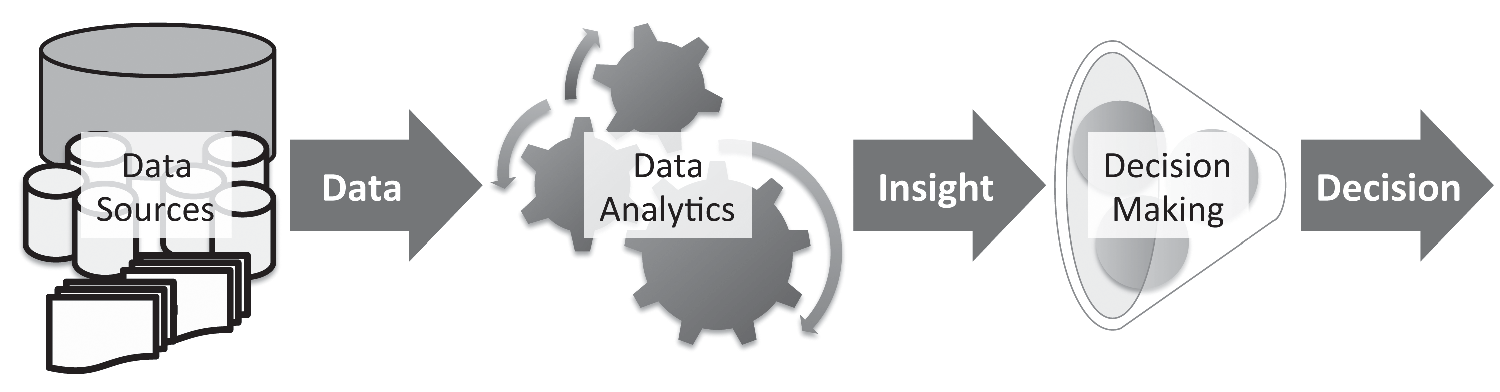
\includegraphics[width=0.95\textwidth]{images/ActionableInsight2_BW.pdf}
       \caption{Predictive data analytics moving from \keyword{data} to \keyword{insights} to \keyword{decisions}.}
     \label{fig:analyticsProcess}
       \end{centering}
\end{figure}
\end{frame} 

\begin{frame} 
\begin{block}{Example Applications:}
	\begin{itemize}
		\item Price Prediction
		\item Fraud Detection
		\item Dosage Prediction
		\item Risk Assessment
		\item Propensity modelling
		\item Diagnosis
		\item Document Classification
		\item $\dots$
	\end{itemize}
\end{block}
\end{frame} 



\SectionSlideShortHeader{What is Machine Learning?}{What is ML?}


\begin{frame}
	\begin{itemize}
		\item (Supervised) Machine Learning techniques automatically learn a model of the relationship between a set of \keyword{descriptive features} and a \keyword{target feature} from a set of historical examples.
	\end{itemize}
\end{frame}

 \begin{frame} [plain]
\begin{figure}[htb]
       \begin{centering}
\includegraphics[width=0.8\textwidth]{images/mlProcessTrain_BW.pdf}
       \caption{Using machine learning to induce a prediction model from a training dataset.}
	\label{fig:mlProcessTrain}
       \end{centering}
\end{figure}
\end{frame} 

 \begin{frame} [plain]
\begin{figure}[htb]
       \begin{centering}
 \includegraphics[width=0.8\textwidth]{images/mlProcessTest_BW.pdf}
       \caption{Using the model to make predictions for new query instances.}
	\label{fig:mlProcessTest}
       \end{centering}
\end{figure}
\end{frame} 



 \begin{frame}[plain]
\begin{table}[htb]
\centering
\begin{tiny}
\resizebox{\textwidth}{!}{\begin{tabular}{ c c  c  c  c }
\hline
\textbf{} & \textbf{\featN{}}	 & \textbf{\featN{}}	& \textbf{\featN{Loan-Salary}} & \textbf{\featN{}}\\
\textbf{ID} & \textbf{\featN{Occupation}}	 & \textbf{\featN{Age}}	& \textbf{\featN{Ratio}} & \textbf{\featN{Outcome}}\\
\hline
1 & industrial	& 34	& 2.96 & repaid \\
2 & professional	& 41	& 4.64	& default \\
3 & professional	& 36	& 3.22	& default \\
4 & professional	& 41	& 3.11	& default \\
5 & industrial	& 48	& 3.80	& default \\
6 & industrial	& 61	& 2.52	& repaid \\
7 & professional	& 37	& 1.50	& repaid \\
8 & professional	& 40	& 1.93	& repaid \\
9 & industrial	& 33	& 5.25	& default \\
10 & industrial	& 32	& 4.15	& default \\
\hline
\end{tabular}
}
\end{tiny}
\end{table}
\begin{itemize}
	\item What is the relationship between the \keyword{descriptive features} (\featN{Occupation}, \featN{Age}, \featN{Loan-Salary Ratio}) and the \keyword{target feature} (\featN{Outcome})?
\end{itemize}
\end{frame} 

\begin{frame}
\begin{center}
\begin{minipage}[t]{0.6\textwidth}
\begin{algorithmic}[0]
	\IF{\featN{Loan-Salary Ratio}$~> 3$}
		\STATE \featN{Outcome}=\featL{default}
        \ELSE 
		\STATE \featN{Outcome}=\featL{repay}
	\ENDIF
\end{algorithmic}
\end{minipage}
\end{center}
\begin{itemize}
	\item<2-4> This is an example of a \keyword{prediction model}
	\item<3-4> This is also an example of a \keyword{consistent} prediction model
	\item<4> Notice that this model does not use all the features and the feature that it uses is a derived feature (in this case a ratio): \keyword{feature design} and \keyword{feature selection} are two important topics that we will return to again and again.
\end{itemize}
\end{frame}

\begin{frame}
\begin{itemize}
	\item What is the relationship between the \keyword{descriptive features} and the \keyword{target feature} (\featN{Outcome}) in the following dataset?
\end{itemize}
\end{frame}

 \begin{frame}[plain] 
\begin{table}[!hb]
\label{table:complexCreditScoringDataset}
\centering
\begin{tiny}
\resizebox{\textwidth}{!}{\begin{tabular}{ c c  c  c  c  c  c  c  c }
\hline
\textbf{}	 &\textbf{}	 & \textbf{}	& \textbf{Loan-}	 & \textbf{} 	 & \textbf{}	 & \textbf{}	 & \textbf{}& \textbf{}\\
\textbf{}	 &\textbf{}	 & \textbf{}	& \textbf{Salary}	 & \textbf{} 	 & \textbf{}	 & \textbf{}	 & \textbf{}& \textbf{}\\
\textbf{ID}	 &\textbf{Amount}	 & \textbf{Salary}	& \textbf{Ratio}	 & \textbf{Age} 	 & \textbf{Occupation}	 & \textbf{House}	 & \textbf{Type}& \textbf{Outcome}\\
\hline
1 & 245,100	 & 	66,400	 & 	3.69	 & 	44	 & 	industrial	 & 	farm	 & 	stb	 & 	repaid	\\
2 & 90,600	 & 	75,300	 & 	1.2	 & 	41	 & 	industrial	 & 	farm	 & 	stb	 & 	repaid	\\
3 & 195,600	 & 	52,100	 & 	3.75	 & 	37	 & 	industrial	 & 	farm	 & 	ftb	 & 	default	\\
4 & 157,800	 & 	67,600	 & 	2.33	 & 	44	 & 	industrial	 & 	apartment	 & 	ftb	 & 	repaid	\\
5 & 150,800	 & 	35,800	 & 	4.21	 & 	39	 & 	professional	 & 	apartment	 & 	stb	 & 	default	\\
6 & 133,000	 & 	45,300	 & 	2.94	 & 	29	 & 	industrial	 & 	farm	 & 	ftb	 & 	default	\\
7 & 193,100	 & 	73,200	 & 	2.64	 & 	38	 & 	professional	 & 	house	 & 	ftb	 & 	repaid	\\
8 & 215,000	 & 	77,600	 & 	2.77	 & 	17	 & 	professional	 & 	farm	 & 	ftb	 & 	repaid	\\
9 & 83,000	 & 	62,500	 & 	1.33	 & 	30	 & 	professional	 & 	house	 & 	ftb	 & 	repaid	\\
10 & 186,100	 & 	49,200	 & 	3.78	 & 	30	 & 	industrial	 & 	house	 & 	ftb	 & 	default	\\
11 & 161,500	 & 	53,300	 & 	3.03	 & 	28	 & 	professional	 & 	apartment	 & 	stb	 & 	repaid	\\
12 & 157,400	 & 	63,900	 & 	2.46	 & 	30	 & 	professional	 & 	farm	 & 	stb	 & 	repaid	\\
13 & 210,000	 & 	54,200	 & 	3.87	 & 	43	 & 	professional	 & 	apartment	 & 	ftb	 & 	repaid	\\
14 & 209,700	 & 	53,000	 & 	3.96	 & 	39	 & 	industrial	 & 	farm	 & 	ftb	 & 	default	\\
15 & 143,200	 & 	65,300	 & 	2.19	 & 	32	 & 	industrial	 & 	apartment	 & 	ftb	 & 	default	\\
16 & 203,000	 & 	64,400	 & 	3.15	 & 	44	 & 	industrial	 & 	farm	 & 	ftb	 & 	repaid	\\
17 & 247,800	 & 	63,800	 & 	3.88	 & 	46	 & 	industrial	 & 	house	 & 	stb	 & 	repaid	\\
18 & 162,700	 & 	77,400	 & 	2.1	 & 	37	 & 	professional	 & 	house	 & 	ftb	 & 	repaid	\\
19 & 213,300	 & 	61,100	 & 	3.49	 & 	21	 & 	industrial	 & 	apartment	 & 	ftb	 & 	default	\\
20 & 284,100	 & 	32,300	 & 	8.8	 & 	51	 & 	industrial	 & 	farm	 & 	ftb	 & 	default	\\
21 & 154,000	 & 	48,900	 & 	3.15	 & 	49	 & 	professional	 & 	house	 & 	stb	 & 	repaid	\\
22 & 112,800	 & 	79,700	 & 	1.42	 & 	41	 & 	professional	 & 	house	 & 	ftb	 & 	repaid	\\
23 & 252,000	 & 	59,700	 & 	4.22	 & 	27	 & 	professional	 & 	house	 & 	stb	 & 	default	\\
24 & 175,200	 & 	39,900	 & 	4.39	 & 	37	 & 	professional	 & 	apartment	 & 	stb	 & 	default	\\
25 & 149,700	 & 	58,600	 & 	2.55	 & 	35	 & 	industrial	 & 	farm	 & 	stb	 & 	default	\\
\hline
\end{tabular}
}
\end{tiny}
\end{table}
\end{frame} 

\begin{frame}
\begin{center}
\begin{minipage}[t]{0.9\textwidth}
\begin{algorithmic}[0]
	\IF{\featN{Loan-Salary Ratio}$~< 1.5$}
		\STATE \featN{Outcome}=\featL{repay}
	\ELSIF{\featN{Loan-Salary Ratio}$~> 4$}
		\STATE \featN{Outcome}=\featL{default}
	\ELSIF{\featN{Age}$~< 40$ \AND \featN{Occupation}$~=$\featL{industrial}}
		\STATE \featN{Outcome}=\featL{default}
        \ELSE 
		\STATE \featN{Outcome}=\featL{repay}
	\ENDIF
\end{algorithmic}
\end{minipage}
\end{center}
\begin{itemize}
	\item<2> \alert{The real value of machine learning becomes apparent in situations like this when we want to build prediction models from large datasets with multiple features.}
\end{itemize}
\end{frame}

\SectionSlideShortHeader{How Does Machine Learning Work?}{How Does ML Work?}

\begin{frame}
\begin{itemize}
	\item<1-3> Machine learning algorithms work by searching through a set of possible prediction models for the model that best captures the relationship between the descriptive features and the target feature.
	\item<2-3> An obvious search criteria to drive this search is to look for models that are \alert{consistent} with the data.
	\item<3> However,  because a training dataset is only a sample ML is an \alert{ill-posed} problem.
	\end{itemize}
\end{frame}

 \begin{frame} 
\begin{table}[htb]
\caption{A simple retail dataset}
\label{table:retailDataset}
\centering
\begin{footnotesize}
\begin{tabular}{ c c c c c }
\hline
\featN{ID}	 & \featN{Bby} 	 & \featN{Alc}	& \featN{Org}  & \featN{Grp} \\
\hline
1	&	no	&	no	&	no	&	couple	\\
2	&	yes	&	no	&	yes	&	family	\\
3	&	yes	&	yes	&	no	&	family	\\
4	&	no	&	no	&	yes	&	couple	\\
5	&	no	&	yes	&	yes	&	single	\\
\hline 
\end{tabular}
\end{footnotesize}
\end{table}
\end{frame} 



 \begin{frame} 
\begin{table}[htb]
\caption{A full set of potential prediction models before any training data becomes available.}
\centering
\begin{tiny}
\resizebox{\textwidth}{!}{\begin{tabular}{c c c | c | c c c c c c c}
\hline
\featN{Bby}	&	\featN{Alc}	&	\featN{Org}	&	~~\featN{Grp}~~	&	$\mathbb{M}_1$	&	$\mathbb{M}_2$	&	$\mathbb{M}_3$	&	$\mathbb{M}_4$	&	$\mathbb{M}_5$	&	\textbf{\dots}	&	$\mathbb{M}_{6\,561}$	\\
\hline																						
no	&	no	&	no	& ?	&	couple		&	couple	&	single	&	couple	&	couple		&	\multirow{8}{*}{\dots}	&	couple	\\
no	&	no	&	yes	&	?	&	single		&	couple	&	single	&	couple	&	couple		&		&	single	\\
no	&	yes	&	no	&	?	&	family	&	family	&	single	&	single	&	single		&		&	family	\\
no	&	yes	&	yes	&	?	&	single	&	single	&	single	&	single	&	single		&		&	couple	\\
yes	&	no	&	no	&	?	&	couple		&	couple	&	family	&	family	&	family		&		&	family	\\
yes	&	no	&	yes	&	?	&	couple		&	family	&	family	&	family	&	family	&		&	couple	\\
yes	&	yes	&	no	&	?	&	single	&	family	&	family	&	family	&	family	&		&	single	\\
yes	&	yes	&	yes	&	?	&	single	&	single	&	family	&	family	&	couple	 &		&	family	\\
\hline
\end{tabular}
}
\end{tiny}
\end{table}
\end{frame} 

 \begin{frame} 
\begin{table}[htb]
\caption{A sample of the models that are consistent with the training data}
\centering
\begin{tiny}
\resizebox{\textwidth}{!}{\begin{tabular}{c c c | c | c c c c c c c}
\hline
\featN{Bby}	&	\featN{Alc}	&	\featN{Org} &	~~\featN{Grp}~~	&	\cellcolor[gray]{0.9} \color{white}{$\mathbb{M}_1$} &	$\mathbb{M}_2$	&	\cellcolor[gray]{0.9} \color{white}{$\mathbb{M}_3$} &	$\mathbb{M}_4$ &	$\mathbb{M}_5$	&	\textbf{\dots}	&	\cellcolor[gray]{0.9} \color{white}{$\mathbb{M}_{6\,561}$}	\\
\hline																						
no	&	no	&	no	& couple	&	\cellcolor[gray]{0.9}\color{white}{couple}	&	couple	&	\cellcolor[gray]{0.9} \color{white}{single}	&	couple	&	couple	 &	\multirow{8}{*}{\dots}	&	\cellcolor[gray]{0.9} \color{white}{couple} \\
no	&	no	&	yes	&	couple	&	\cellcolor[gray]{0.9}\color{white}{single}	&	couple	&	\cellcolor[gray]{0.9} \color{white}{single} &	couple	&	couple	&		&	\cellcolor[gray]{0.9} \color{white}{single}	\\
no	&	yes	&	no	&	?	&	\cellcolor[gray]{0.9}\color{white}{family}	&	family	&	\cellcolor[gray]{0.9} \color{white}{single} 	&	single	&	single	&		& \cellcolor[gray]{0.9} \color{white}{family}	\\
no	&	yes	&	yes	&	single	&	\cellcolor[gray]{0.9}\color{white}{single}	&	single	&	\cellcolor[gray]{0.9} \color{white}{single} 	&	single	&	single	&		&	\cellcolor[gray]{0.9} \color{white}{couple} \\
yes	&	no	&	no	&	?	&	\cellcolor[gray]{0.9}\color{white}{couple}	&	couple	&	\cellcolor[gray]{0.9} \color{white}{family} &	family	&	family	&		&	\cellcolor[gray]{0.9} \color{white}{family} 	\\
yes	&	no	&	yes	&	family	&	\cellcolor[gray]{0.9}\color{white}{couple}	&	family	&	\cellcolor[gray]{0.9} \color{white}{family} &	family	&	family	&		&	\cellcolor[gray]{0.9} \color{white}{couple} 	\\
yes	&	yes	&	no	&	family	&	\cellcolor[gray]{0.9}\color{white}{single}	&	family	&	\cellcolor[gray]{0.9} \color{white}{family} &	family	&	family	&		&	\cellcolor[gray]{0.9} \color{white}{single} 	\\
yes	&	yes	&	yes	&	?	&	\cellcolor[gray]{0.9}\color{white}{single} &	single	&	\cellcolor[gray]{0.9} \color{white}{family} &	family	&	couple &		&	\cellcolor[gray]{0.9} \color{white}{family} 	\\
\hline
\end{tabular}
}
\end{tiny}
\end{table}
\begin{itemize}
	\item<2> Notice that there is more than one candidate model left! It is because a single consistent model cannot be found based on a \alert{sample} training dataset that ML is \alert{ill-posed}.
\end{itemize}
\end{frame} 

\begin{frame}
	\begin{itemize}
		\item Consistency $\approx$ \alert{memorizing} the dataset. 
		\item Consistency with  \alert{noise} in the data isn't desirable.
		\item Goal: a model that \keyword{generalises} beyond the dataset and that isn't influenced by the noise in the dataset.
		\item So what criteria should we use for choosing between models?
	\end{itemize}
\end{frame}

\begin{frame}
		\begin{itemize}
			\item \alert{Inductive bias} the set of assumptions that define the model selection criteria of an ML algorithm.
			\item There are two types of bias that we can use:
			\begin{enumerate}
					\item restriction bias
					\item preference bias
			\end{enumerate}
			\item Inductive bias is necessary for learning (beyond the dataset).
		\end{itemize}
\end{frame}

\begin{frame}
	\begin{block}{How ML works (Summary)}
	\begin{itemize}
		\item ML algorithms work by searching through sets of potential models.
		\item There are two sources of information that guide this search:
			\begin{enumerate}
				\item the training data,
				\item the inductive bias of the algorithm.
			\end{enumerate}
	\end{itemize}
	\end{block}
\end{frame}

\SectionSlideShortHeader{Inductive Bias Versus Sample Bias}{Bias}

\begin{frame}
	\begin{itemize}
		\item Inductive bias is necessary for machine learning, and in a sense, a key goal of a data analyst is to find the correct inductive bias.
		\item Inductive bias is not the only type of bias that affects machine learning, a particularly important type of bias that we need to be aware of is \keyword{sampling bias}	
	\end{itemize}
\end{frame}

\begin{frame}
	\begin{itemize}
		\item Sampling bias arises when the sample of data used within a data-driven process is collected in such a way that the sample is not representative of the population the sample is used to represent. 
		\item  If a sample of data is not representative of a population, then inferences based on that sample will not generalize to the larger population. 
		\item Sample bias is something that a data analyst should proactively work hard to remove from the data used in any data analytics project.		
	\end{itemize}
\end{frame}

\SectionSlideShortHeader{What Can Go Wrong With ML?}{Underfitting/Overfitting}

\begin{frame}
	\begin{itemize}
			\item No free lunch!
			\item What happens if we choose the wrong inductive bias: 
			\begin{enumerate}
				\item \keyword{underfitting}
				\item \keyword{overfitting}
			\end{enumerate}
	\end{itemize}
\end{frame}

 \begin{frame} 
\begin{table}[!tb]
\caption{The age-income dataset.}
\label{table:incomeAgeTable}
\centering
\begin{footnotesize}
\begin{tabular}{ c  c  c }
\hline
\featN{ID}	 & \featN{Age}	& \featN{Income} \\
\hline
1	 & 21	 & 24,000	 \\
2	 & 32	 & 48,000	 \\
3	 & 62	 & 83,000	 \\
4	 & 72	 & 61,000	 \\
5	 & 84	 & 52,000	 \\
\hline
\end{tabular}
\end{footnotesize}
\end{table}
\end{frame} 

 \begin{frame} 
\begin{figure}[!htb]
       \begin{centering}
	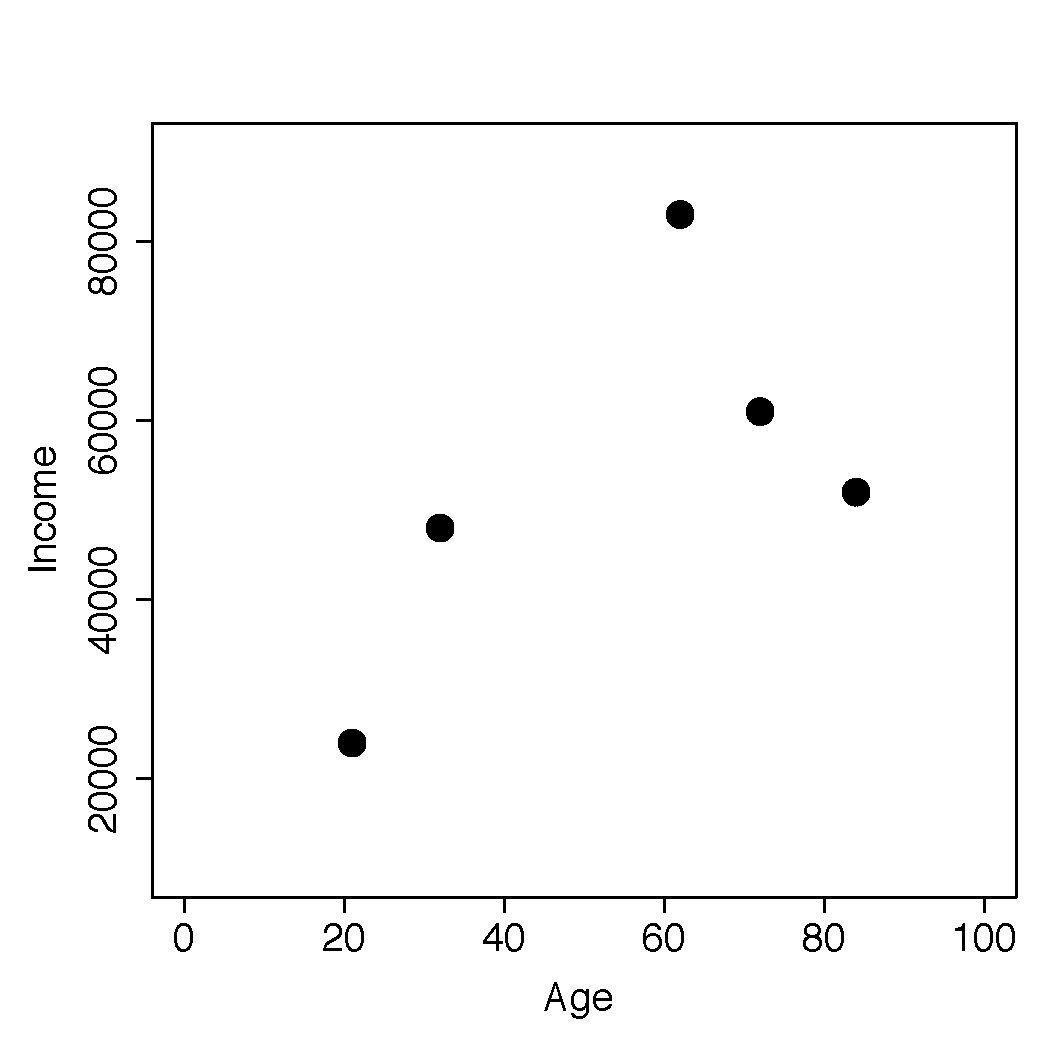
\includegraphics[width=0.7\textwidth]{images/IntroOverfittingUnderfittingPlot1.pdf}
       \label{fig:ageIncome}
       \end{centering}
\end{figure}
\end{frame}



 \begin{frame} 
\begin{figure}[!htb]
       \begin{centering}
	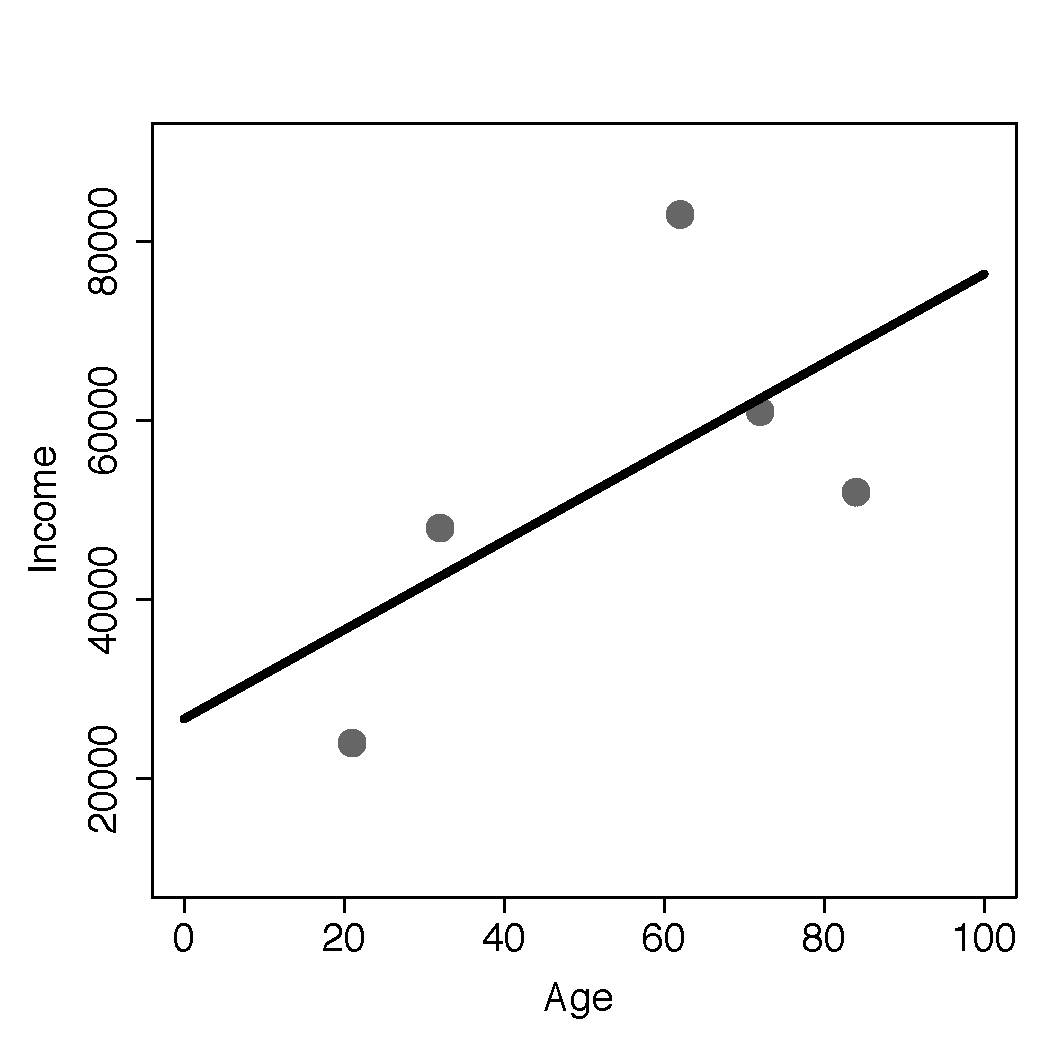
\includegraphics[width=0.7\textwidth]{images/IntroOverfittingUnderfittingPlot2.pdf}
       \label{fig:ageIncome}
       \end{centering}
\end{figure}

\end{frame} 


 \begin{frame} 

\begin{figure}[!htb]
       \begin{centering}
	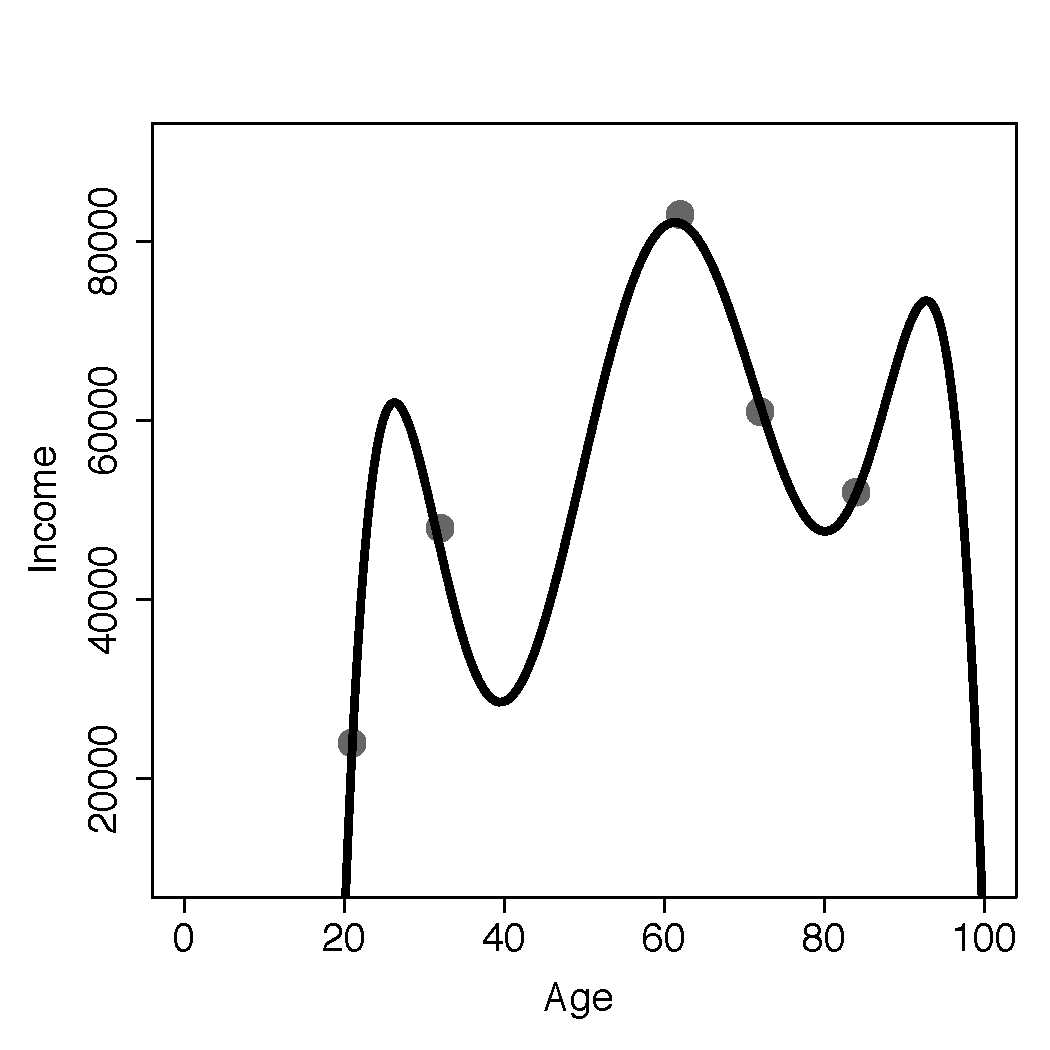
\includegraphics[width=0.7\textwidth]{images/IntroOverfittingUnderfittingPlot4.pdf}
       \label{fig:ageIncome}
       \end{centering}
\end{figure}

\end{frame} 

 \begin{frame} 

\begin{figure}[!htb]
       \begin{centering}
	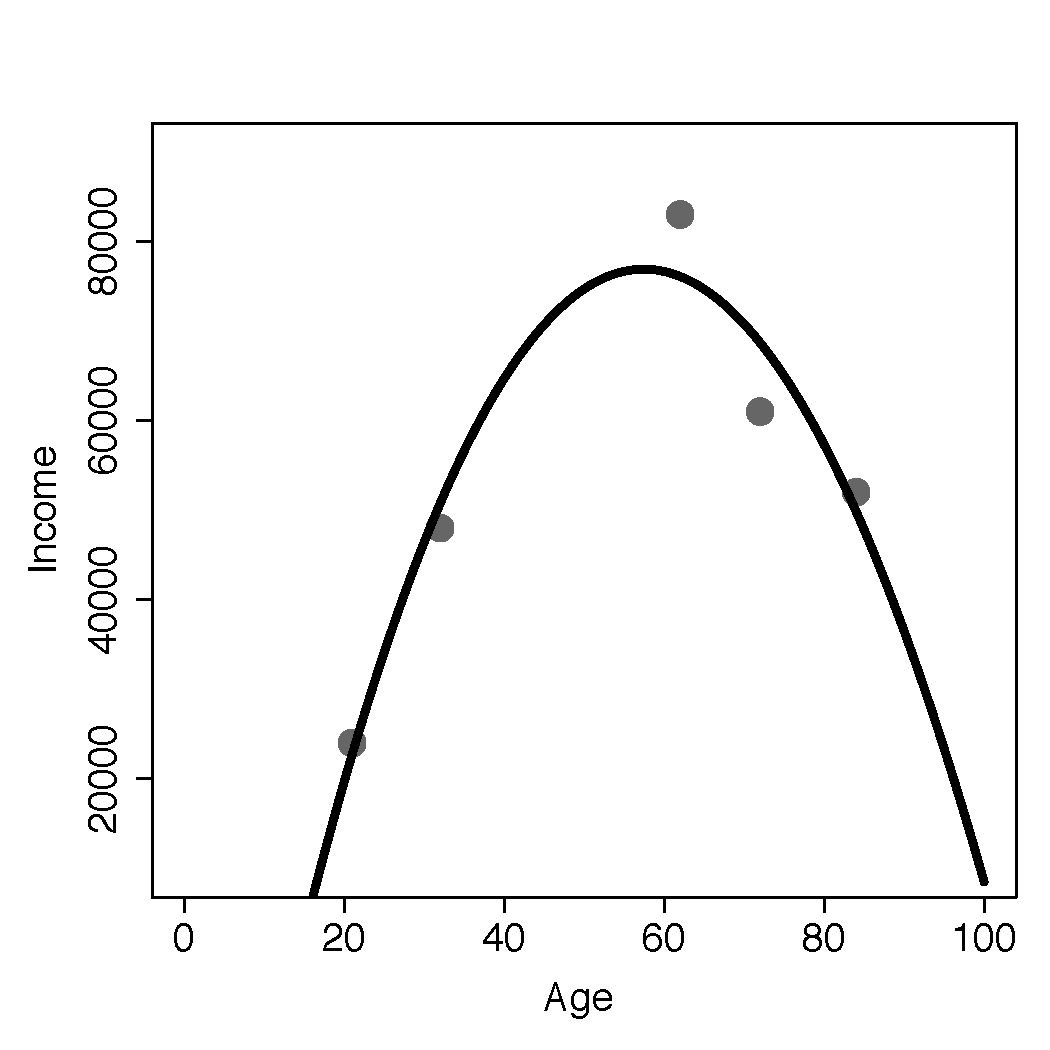
\includegraphics[width=0.7\textwidth]{images/IntroOverfittingUnderfittingPlot3.pdf}
       \label{fig:ageIncome}
       \end{centering}
\end{figure}

\end{frame} 



 \begin{frame} 
\begin{figure}[!htb]
       \begin{centering}
       	\subfigure[Dataset]{\label{fig:overfittingUnderfittingA}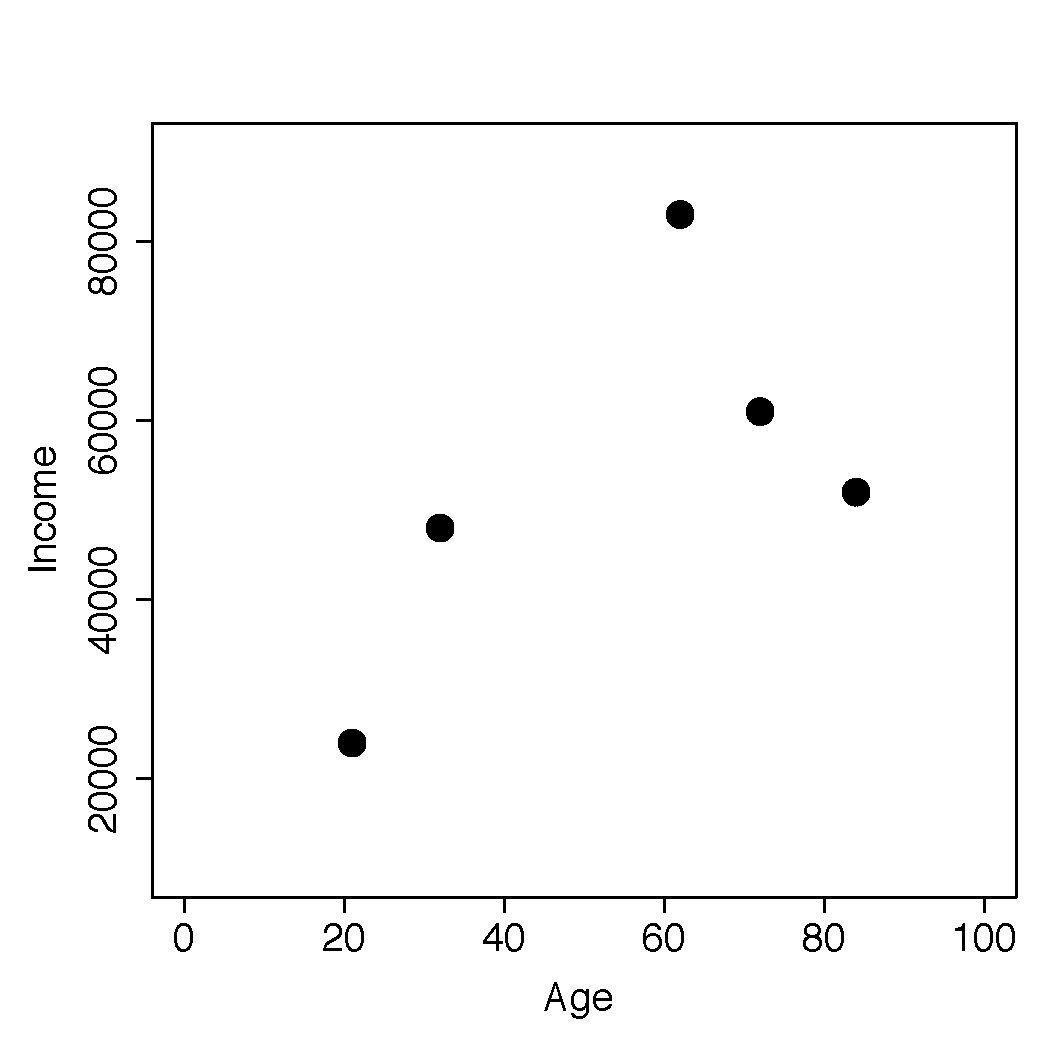
\includegraphics[width=0.22\textwidth]{images/IntroOverfittingUnderfittingPlot1.pdf}}
      	\subfigure[Underfitting]{\label{fig:overfittingUnderfittingB}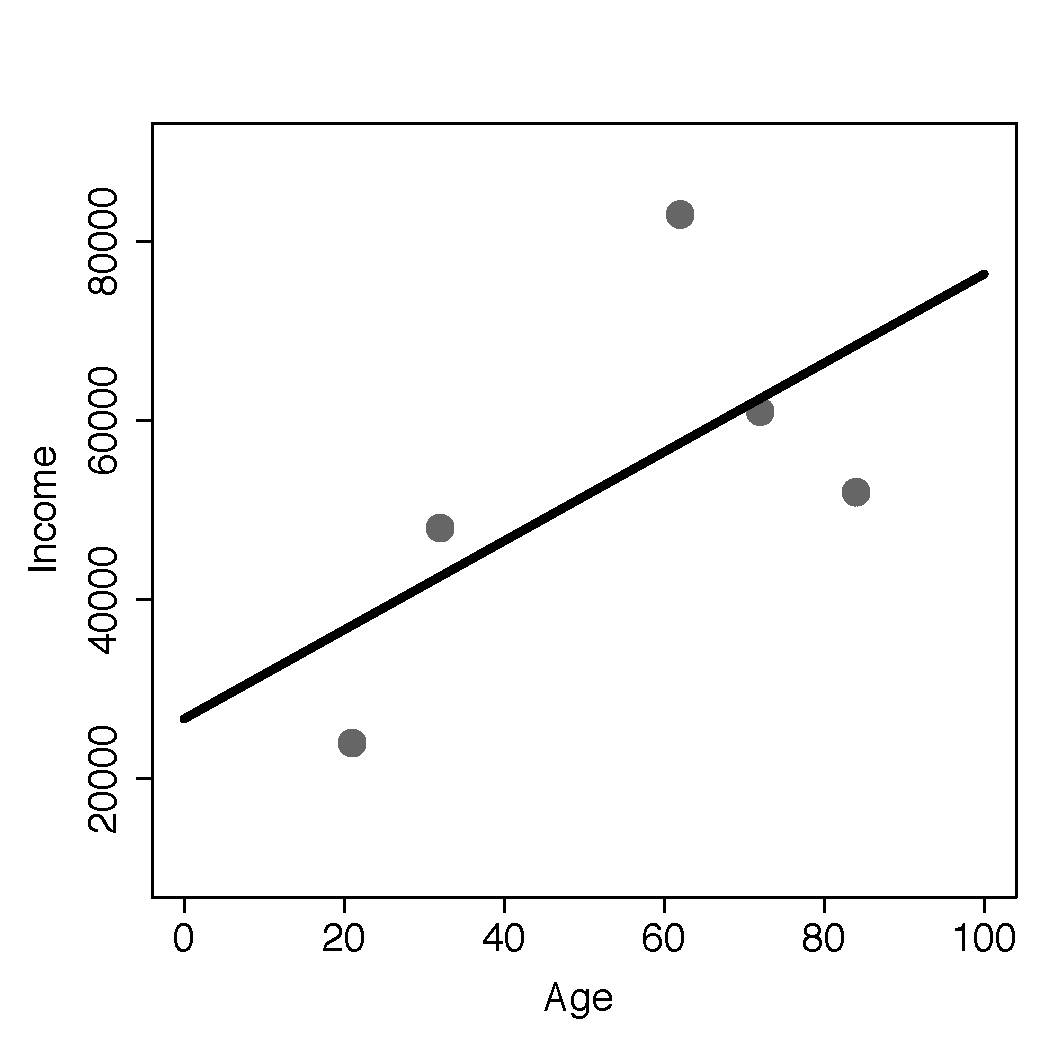
\includegraphics[width=0.22\textwidth]{images/IntroOverfittingUnderfittingPlot2.pdf}}
       	\subfigure[Overfitting]{\label{fig:overfittingUnderfittingD}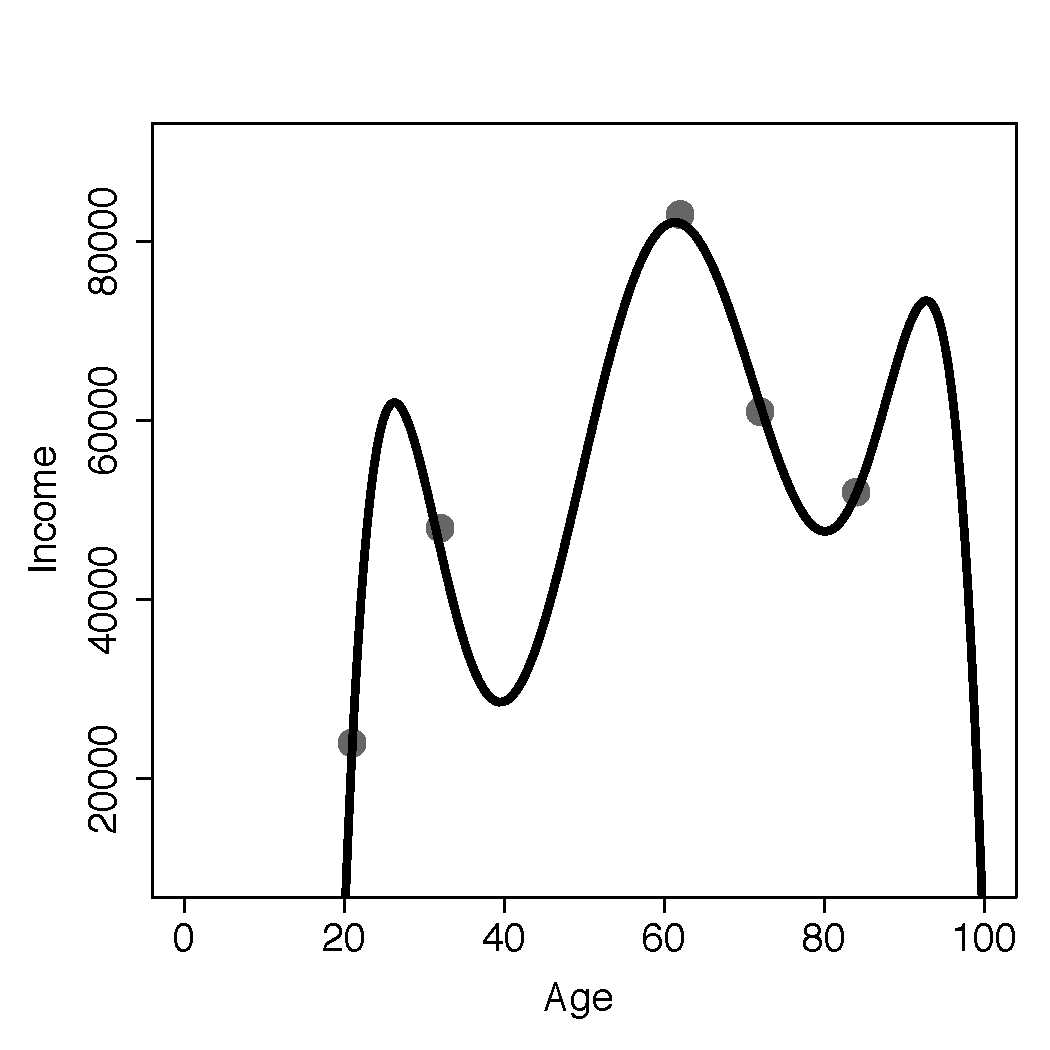
\includegraphics[width=0.22\textwidth]{images/IntroOverfittingUnderfittingPlot4.pdf}}
       	\subfigure[Just right]{\label{fig:overfittingUnderfittingC}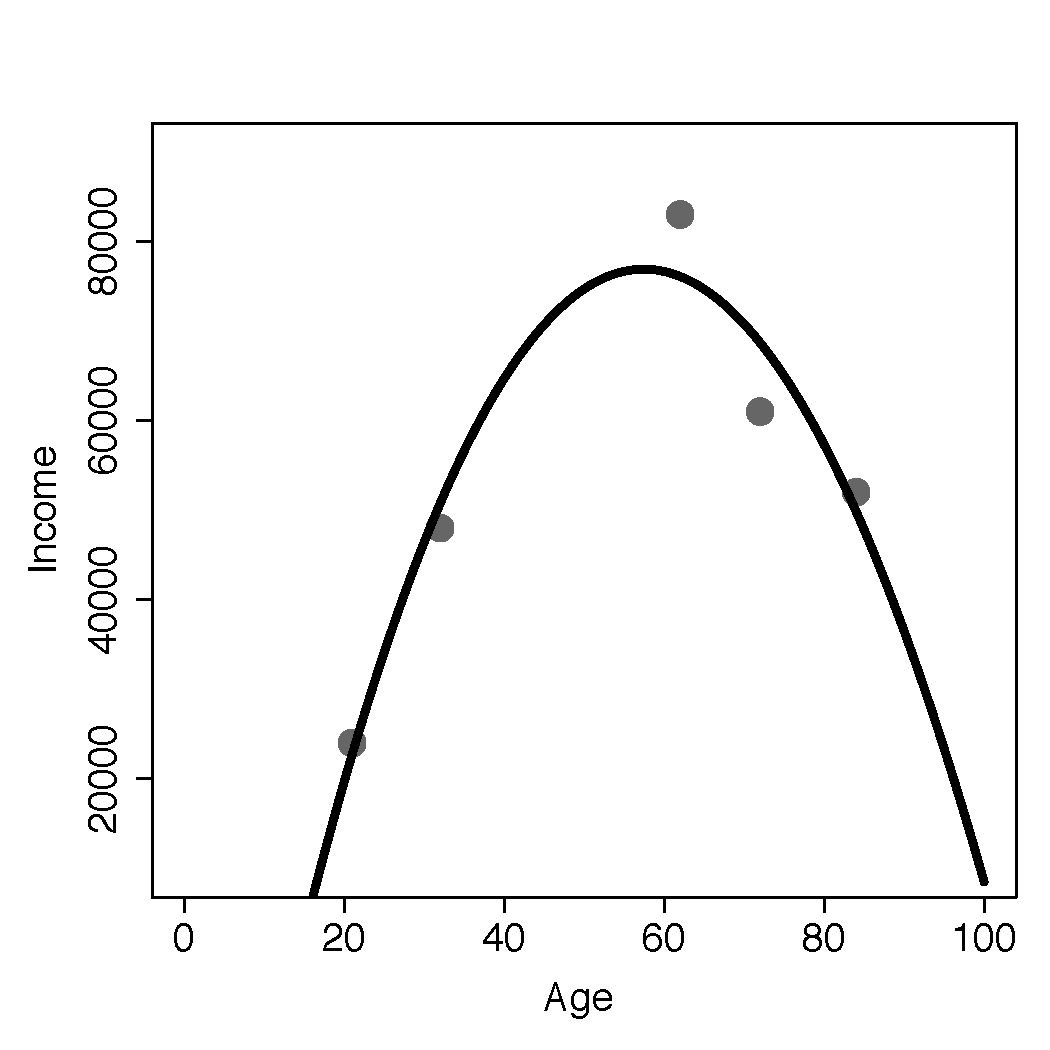
\includegraphics[width=0.22\textwidth]{images/IntroOverfittingUnderfittingPlot3.pdf}}
       \caption{Striking a balance between overfitting and underfitting when trying to predict age from income.}
       \label{fig:overfittingUnderfitting}
       \end{centering}
\end{figure}
\end{frame} 

\SectionSlideShortHeader{The Predictive Data Analytics Project Lifecycle: Crisp-DM}{Lifecycle}

 \begin{frame} [plain]
\begin{figure}[!htb]
	\begin{center}
			\includegraphics[width=0.7\textwidth]{./images/CrispDM_BW_mod.pdf}
	\end{center}
	\caption{A diagram of the CRISP-DM process which shows the six key phases and indicates the important relationships between them. This figure is based on Figure 2 of \cite{wirth2000crisp}.}
	\label{fig:crispDM}
\end{figure}
\end{frame} 

\SectionSlideShortHeader{The Road Ahead}{Road Ahead}

\begin{frame}
	\begin{itemize}
		\item Part 1 of the course will cover the preparatory activity prior to model building.
			\begin{enumerate}
				\item Business Understanding
				\item Data Understanding
				\item Data Preparation
			\end{enumerate}
\end{itemize}
\end{frame}

\begin{frame}
	\begin{itemize}
		\item Part II focuses on five families of machine learning algorithms for predictive data analytics:
			\begin{enumerate}
				\item \keyword{Information based learning}
				\item \keyword{Similarity based learning}
				\item \keyword{Probability based learning}
				\item \keyword{Error based learning}
				\item \keyword{Deep Learning}
			\end{enumerate}
		\item We also cover a range of approaches to evaluating prediction models.
	\end{itemize}
\end{frame}

\begin{frame}
	\begin{itemize}
		\item Part III also deals with modelling but looks at modelling approaches beyond prediction
			\begin{enumerate}
				\item \keyword{Unsupervised Learning}
				\item \keyword{Reinforcement learning}
			\end{enumerate}
		\item Par IV covers questions relating deployment and includes case studies that illustrate how everything described in the preceding sections come together in a successful predictive data analytics project.
	\end{itemize}
\end{frame}




\SectionSlide{Summary}

\begin{frame}
\begin{itemize}
	\item Machine Learning techniques automatically learn the relationship between a set of \keyword{descriptive features} and a \keyword{target feature} from a set of historical examples.
	\item Machine Learning is an \keyword{ill-posed} problem: 
			\begin{enumerate}
				\item \keyword{generalize}, 
				\item \keyword{inductive bias}, 
				\item \keyword{underfitting}, 
				\item \keyword{overfitting}.
			\end{enumerate}
	\item Striking the right balance between model complexity and simplicity (between underfitting and overfitting) is the hardest part of machine learning.
\end{itemize}
\end{frame}

\begin{frame}[allowframebreaks]
        \tiny{\bibliographystyle{abbrv}}
        \bibliography{Book}
\end{frame}

\begin{frame}
	\tableofcontents
\end{frame}



\end{document}
